\paragraph{Sơ đồ tuần tự Luồng Cấp token voice chat qua LiveKit}

Luồng này mô tả quá trình Web Frontend xin Access Token để người dùng tham gia phòng voice chat trên LiveKit. Conversation Service kiểm tra quyền VIP khi không chạy ở môi trường \texttt{development}, tạo token bằng LiveKit SDK và nhúng metadata để Voice Agent sử dụng khi xử lý cuộc trò chuyện.

\begin{figure}[H]
\centering
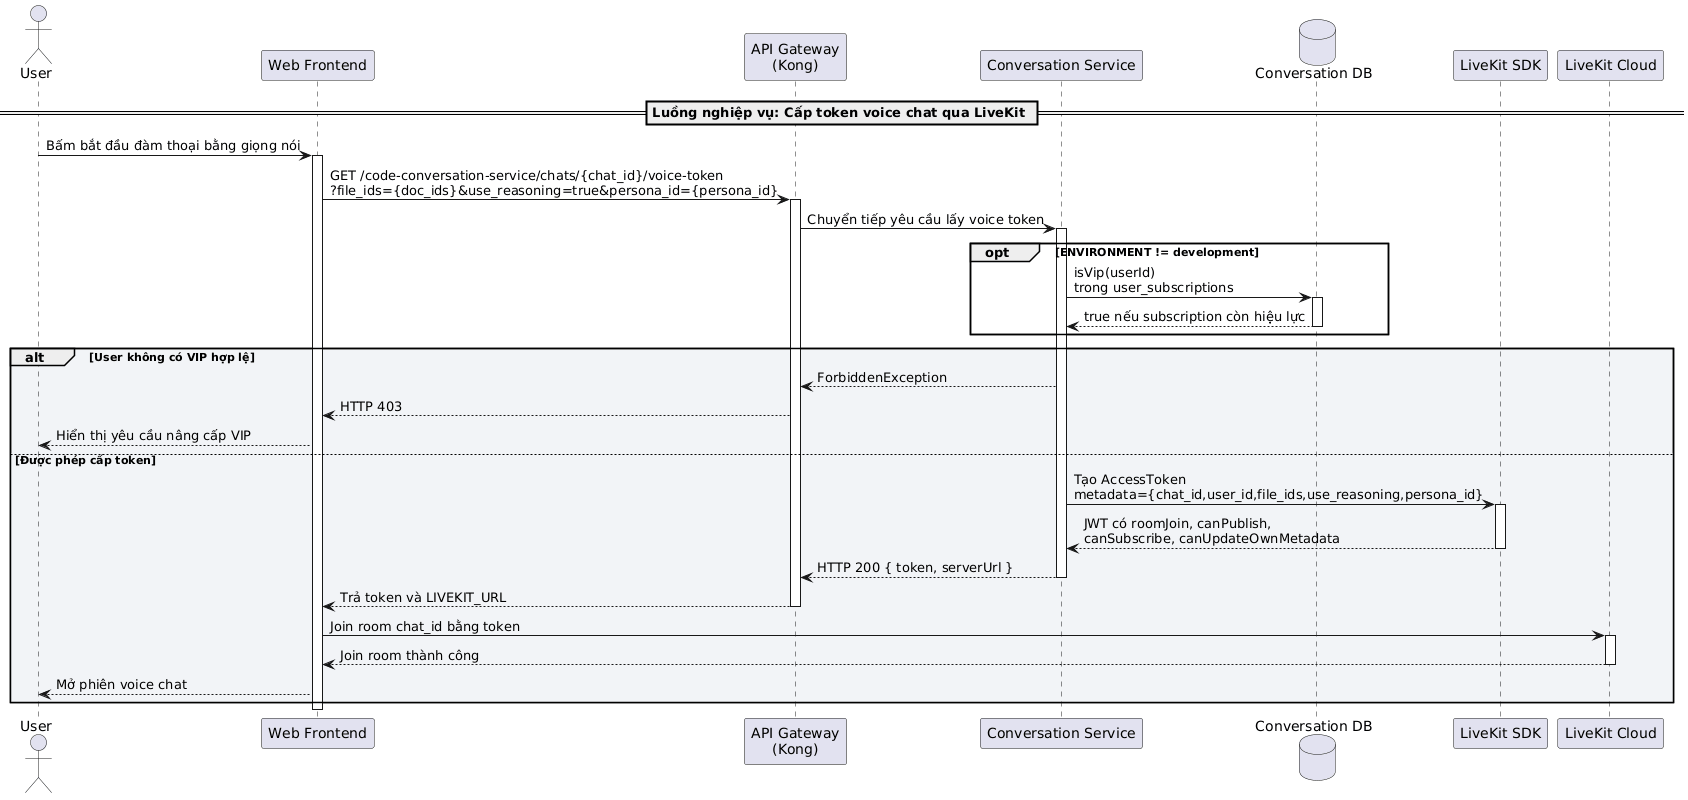
\includegraphics[scale = 0.18]{contents/Sequence/UML-Sequence-UserVoiceLiveKitToken.png}
\caption{Sơ đồ tuần tự Luồng Cấp token voice chat qua LiveKit}
\end{figure}

\subparagraph{Các thành phần tham gia}

\begin{table}[H]
\centering
\renewcommand{\arraystretch}{1.3}
\begin{tabular}{|l|l|p{5cm}|}
\hline
\textbf{Thành phần} & \textbf{Phân loại} & \textbf{Vai trò trong hệ thống} \\ \hline
User & Actor & Người dùng bắt đầu phiên voice chat. \\ \hline
Web Frontend & Component & Giao diện web Next.js. \\ \hline %%%% Component & Gọi API lấy token và kết nối tới LiveKit Cloud. \\ \hline
API Gateway (Kong) & Component & Định tuyến request tới Conversation Service. \\ \hline
Conversation Service & Microservice & Kiểm tra VIP và tạo Access Token bằng LiveKit SDK. \\ \hline
Conversation Database & Database & Lưu trạng thái subscription được đồng bộ từ Payment Service. \\ \hline
LiveKit Cloud & External Service & Hạ tầng WebRTC/WebSocket cho phiên đàm thoại thời gian thực. \\ \hline
\end{tabular}
\caption{Các thành phần tham gia luồng cấp token voice chat qua LiveKit}
\end{table}

\subparagraph{Mô tả chi tiết}
\begin{itemize}
\item Web Frontend gọi \texttt{GET /code-conversation-service/chats/\{chat\_id\}/voice-token} kèm \texttt{file\_ids[]}, \texttt{use\_reasoning} và \texttt{persona\_id}.
\item Conversation Service kiểm tra VIP khi môi trường khác \texttt{development}; nếu không hợp lệ thì trả \texttt{ForbiddenException}.
\item Access Token chứa metadata \texttt{chat\_id}, \texttt{user\_id}, \texttt{file\_ids}, \texttt{use\_reasoning} và \texttt{persona\_id}.
\item Token có quyền \texttt{roomJoin}, \texttt{canPublish}, \texttt{canSubscribe} và \texttt{canUpdateOwnMetadata}. Client dùng token và \texttt{LIVEKIT\_URL} để join room tương ứng với \texttt{chat\_id}.
\end{itemize}
